\chapter{Algoritmos de barrido}

\index{algoritmo!de barrido}
\indexaltsub{algoritmo}{sweep line}

Muchos problemas geométricos pueden resolverse utilizando \key{algoritmos de
    barrido}. La idea principal de estos algoritmos es representar una instancia
del problema como un conjunto de eventos que corresponden a puntos en el
plano. Los eventos se procesan en orden creciente acorde a sus coordenadas
$x$ o $y$.

Por ejemplo, considera el siguiente problema: hay una compañía con $n$
empleados y sabemos, para cada empleado, su hora de llegada y partida en
un cierto día. Nuestra tarea es calcular el número máximo de empleados que
estuvieron en la oficina simultáneamente.

Podemos resolver el problema modelando la situación tal que cada empleado
es asignado dos eventos que corresponden a sus horas de llegada y partida.
Luego de ordenar los eventos, los recorremos y mantenemos registro del
número de gente en la oficina. Por ejemplo, la tabla
\begin{center}
    \begin{tabular}{ccc}
        empleado & llegada & partida \\
        \hline
        Juan     & 10      & 15      \\
        María    & 6       & 12      \\
        Pedro    & 14      & 16      \\
        Lisa     & 5       & 13      \\
    \end{tabular}
\end{center}
corresponde a los siguientes eventos:
\begin{center}
    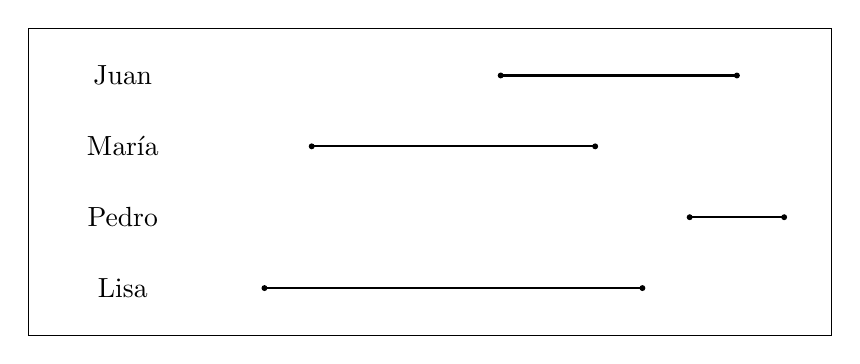
\begin{tikzpicture}[scale=0.6]
        \draw (0,0) rectangle (17,-6.5);
        \path[draw,thick,-] (10,-1) -- (15,-1);
        \path[draw,thick,-] (6,-2.5) -- (12,-2.5);
        \path[draw,thick,-] (14,-4) -- (16,-4);
        \path[draw,thick,-] (5,-5.5) -- (13,-5.5);

        \draw[fill] (10,-1) circle [radius=0.05];
        \draw[fill] (15,-1) circle [radius=0.05];
        \draw[fill] (6,-2.5) circle [radius=0.05];
        \draw[fill] (12,-2.5) circle [radius=0.05];
        \draw[fill] (14,-4) circle [radius=0.05];
        \draw[fill] (16,-4) circle [radius=0.05];
        \draw[fill] (5,-5.5) circle [radius=0.05];
        \draw[fill] (13,-5.5) circle [radius=0.05];

        \node at (2,-1) {Juan};
        \node at (2,-2.5) {María};
        \node at (2,-4) {Pedro};
        \node at (2,-5.5) {Lisa};
    \end{tikzpicture}
\end{center}
Recorremos los eventos de izquierda a derecha y mantenemos un contador. Cada
vez que llega una persona, incrementamos el contador, y cuando una persona
parte, decrementamos el contador. La respuesta al problema es el máximo
valor del contador durante la ejecución.

En el ejemplo, los eventos se procesan en este orden:
\begin{center}
    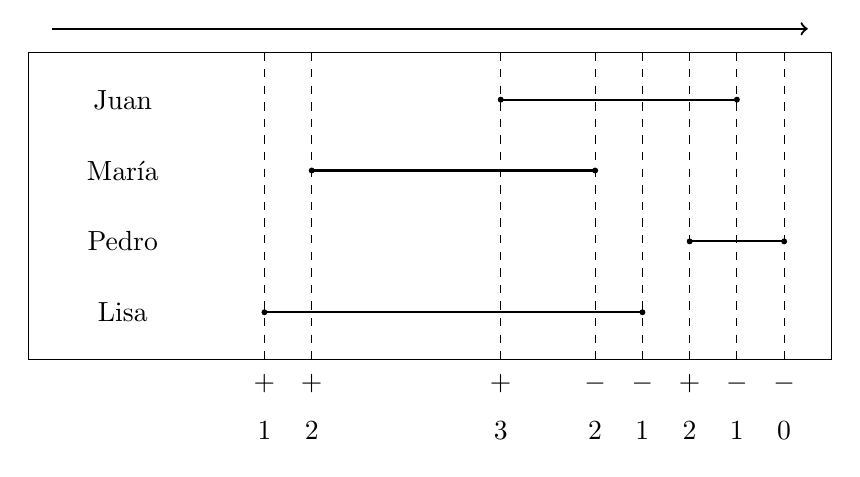
\begin{tikzpicture}[scale=0.6]
        \path[draw,thick,->] (0.5,0.5) -- (16.5,0.5);
        \draw (0,0) rectangle (17,-6.5);
        \path[draw,thick,-] (10,-1) -- (15,-1);
        \path[draw,thick,-] (6,-2.5) -- (12,-2.5);
        \path[draw,thick,-] (14,-4) -- (16,-4);
        \path[draw,thick,-] (5,-5.5) -- (13,-5.5);

        \draw[fill] (10,-1) circle [radius=0.05];
        \draw[fill] (15,-1) circle [radius=0.05];
        \draw[fill] (6,-2.5) circle [radius=0.05];
        \draw[fill] (12,-2.5) circle [radius=0.05];
        \draw[fill] (14,-4) circle [radius=0.05];
        \draw[fill] (16,-4) circle [radius=0.05];
        \draw[fill] (5,-5.5) circle [radius=0.05];
        \draw[fill] (13,-5.5) circle [radius=0.05];

        \node at (2,-1) {Juan};
        \node at (2,-2.5) {María};
        \node at (2,-4) {Pedro};
        \node at (2,-5.5) {Lisa};

        \path[draw,dashed] (10,0)--(10,-6.5);
        \path[draw,dashed] (15,0)--(15,-6.5);
        \path[draw,dashed] (6,0)--(6,-6.5);
        \path[draw,dashed] (12,0)--(12,-6.5);
        \path[draw,dashed] (14,0)--(14,-6.5);
        \path[draw,dashed] (16,0)--(16,-6.5);
        \path[draw,dashed] (5,0)--(5,-6.5);
        \path[draw,dashed] (13,0)--(13,-6.5);

        \node at (10,-7) {$+$};
        \node at (15,-7) {$-$};
        \node at (6,-7) {$+$};
        \node at (12,-7) {$-$};
        \node at (14,-7) {$+$};
        \node at (16,-7) {$-$};
        \node at (5,-7) {$+$};
        \node at (13,-7) {$-$};

        \node at (10,-8) {$3$};
        \node at (15,-8) {$1$};
        \node at (6,-8) {$2$};
        \node at (12,-8) {$2$};
        \node at (14,-8) {$2$};
        \node at (16,-8) {$0$};
        \node at (5,-8) {$1$};
        \node at (13,-8) {$1$};
    \end{tikzpicture}
\end{center}
Los símbolos $+$ y $-$ indican si el valor del contador aumenta o disminuye,
y el valor del contador se muestra debajo. El valor máximo del contador fue
3, entre la llegada de Juan y la partida de María.

La complejidad temporal del algoritmo es de $O(n \log n)$, porque ordenar los
eventos tarda $O(n \log n)$ y el resto del algoritmo tarda $O(n)$.

\section{Puntos de intersección}

\index{punto de intersección}

Dado un conjunto de $n$ segmentos, cada uno siendo horizontal o vertical,
considera el problema de contar el número total de puntos de intersección.
Por ejemplo, cuando los segmentos son
\begin{center}
    \begin{tikzpicture}[scale=0.5]
        \path[draw,thick,-] (0,2) -- (5,2);
        \path[draw,thick,-] (1,4) -- (6,4);
        \path[draw,thick,-] (6,3) -- (10,3);
        \path[draw,thick,-] (2,1) -- (2,6);
        \path[draw,thick,-] (8,2) -- (8,5);
    \end{tikzpicture}
\end{center}
existen tres puntos de intersección:
\begin{center}
    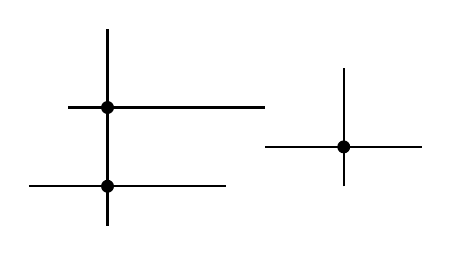
\begin{tikzpicture}[scale=0.5]
        \path[draw,thick,-] (0,2) -- (5,2);
        \path[draw,thick,-] (1,4) -- (6,4);
        \path[draw,thick,-] (6,3) -- (10,3);
        \path[draw,thick,-] (2,1) -- (2,6);
        \path[draw,thick,-] (8,2) -- (8,5);

        \draw[fill] (2,2) circle [radius=0.15];
        \draw[fill] (2,4) circle [radius=0.15];
        \draw[fill] (8,3) circle [radius=0.15];

    \end{tikzpicture}
\end{center}

Es fácil resolver el problema en $O(n^2)$, porque podemos recorrer todos los
pares posibles de segmentos y revisar si se intersecan. Sin embargo, podemos
resolver este problema eficientemente en $O(n \log n)$ usando un algoritmo de
barrido y una estructura de datos para consultas en rango.

La idea es procesar los extremos de los segmentos de izquierda a derecha y
concentrarnos en tres tipos de eventos:
\begin{enumerate}[noitemsep]
    \item[(1)] segmento horizontal comienza
    \item[(2)] segmento horizontal termina
    \item[(3)] segmento vertical aparece
\end{enumerate}

Los siguientes eventos corresponden al ejemplo:
\begin{center}
    \begin{tikzpicture}[scale=0.6]
        \path[draw,dashed] (0,2) -- (5,2);
        \path[draw,dashed] (1,4) -- (6,4);
        \path[draw,dashed] (6,3) -- (10,3);
        \path[draw,dashed] (2,1) -- (2,6);
        \path[draw,dashed] (8,2) -- (8,5);

        \node at (0,2) {$1$};
        \node at (5,2) {$2$};
        \node at (1,4) {$1$};
        \node at (6,4) {$2$};
        \node at (6,3) {$1$};
        \node at (10,3) {$2$};

        \node at (2,3.5) {$3$};
        \node at (8,3.5) {$3$};
    \end{tikzpicture}
\end{center}

Recorremos los eventos de izquierda a derecha y utilizamos una estructura de
datos que mantiene un conjunto de coordenadas $y$ donde haya algún segmento
horizontal activo. En el evento 1, añadimos la coordenada $y$ del segmento al
conjunto, y en el evento 2, removemos la coordenada $y$ del conjunto.

Los puntos de intersección se calculan en el evento 3. Cuando hay un segmento
vertical entre los puntos $y_1$ e $y_2$, contamos el numero de segmentos
horizontales activos cuyas coordenadas $y$ se encuentren entre $y_1$ e $y_2$,
y añadimos este número al total de puntos de intersección.

Para almacenar las coordenadas $y$ de segmentos horizontales, podemos utilizar
un árbol binario indexado o de segmentos, posiblemente con compresión de
índices. Al usar estas estructuras, procesar cada evento tarda $O(\log n)$,
por lo que el tiempo total de ejecución del algoritmo es $O(n \log n)$.

\section{Par más cercano}

\index{par más cercano}

Dado un conjunto de $n$ puntos, nuestro siguiente problema es encontrar dos
puntos cuya distancia euclideana sea mínima. Por ejemplo, si los puntos son
\begin{center}
    \begin{tikzpicture}[scale=0.7]
        \draw (0,0)--(12,0)--(12,4)--(0,4)--(0,0);

        \draw (1,2) circle [radius=0.1];
        \draw (3,1) circle [radius=0.1];
        \draw (4,3) circle [radius=0.1];
        \draw (5.5,1.5) circle [radius=0.1];
        \draw (6,2.5) circle [radius=0.1];
        \draw (7,1) circle [radius=0.1];
        \draw (9,1.5) circle [radius=0.1];
        \draw (10,2) circle [radius=0.1];
        \draw (1.5,3.5) circle [radius=0.1];
        \draw (1.5,1) circle [radius=0.1];
        \draw (2.5,3) circle [radius=0.1];
        \draw (4.5,1.5) circle [radius=0.1];
        \draw (5.25,0.5) circle [radius=0.1];
        \draw (6.5,2) circle [radius=0.1];
    \end{tikzpicture}
\end{center}
deberíamos encontrar los siguientes puntos:
\begin{center}
    \begin{tikzpicture}[scale=0.7]
        \draw (0,0)--(12,0)--(12,4)--(0,4)--(0,0);

        \draw (1,2) circle [radius=0.1];
        \draw (3,1) circle [radius=0.1];
        \draw (4,3) circle [radius=0.1];
        \draw (5.5,1.5) circle [radius=0.1];
        \draw[fill] (6,2.5) circle [radius=0.1];
        \draw (7,1) circle [radius=0.1];
        \draw (9,1.5) circle [radius=0.1];
        \draw (10,2) circle [radius=0.1];
        \draw (1.5,3.5) circle [radius=0.1];
        \draw (1.5,1) circle [radius=0.1];
        \draw (2.5,3) circle [radius=0.1];
        \draw (4.5,1.5) circle [radius=0.1];
        \draw (5.25,0.5) circle [radius=0.1];
        \draw[fill] (6.5,2) circle [radius=0.1];
    \end{tikzpicture}
\end{center}


Este es otro ejemplo de un problema que puede resolverse en $O(n \log n)$
utilizando un algoritmo de barrido.\footnote{Aparte de este método, también
    existe un algoritmo \textit{divide y vencerás} de tiempo $O(n \log n)$
    \cite{sha75} que divide los puntos en dos conjuntos y resuelve el
    problema recursivamente para ambos.}
Recorremos los puntos de izquierda a derecha y mantenemos un valor $d$: la
minima distancia entre dos puntos vistos hasta ahora. En cada punto,
encontramos el punto más cercano a la izquierda. Si la distancia es menor
que $d$, es la nueva mínima distancia y actualizamos el valor de $d$.

Si el punto actual es $(x,y)$ y existe un punto a la izquierda dentro de una
distancia menor que $d$, la coordenada $x$ de un punto tal debe estar entre
$[x-d,x]$ y la coordenada $y$ debe estar entre $[y-d,y+d]$. Por lo tanto,
podemos solamente considerar puntos dentro de esos rangos, lo que hace al
algoritmo eficiente.

Por ejemplo, en la siguiente imagen, la región marcada con lineas punteadas
contiene los puntos que pueden estar a una distancia de $d$ desde el punto
activo:

\begin{center}
    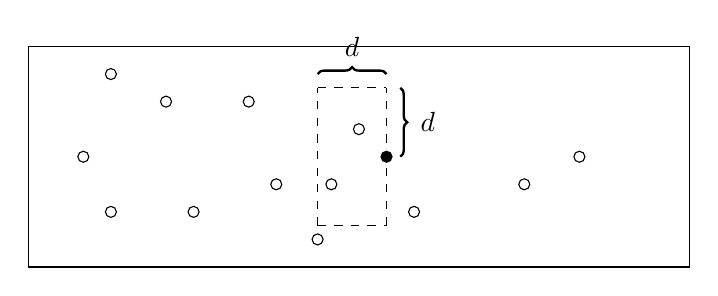
\begin{tikzpicture}[scale=0.7]
        \draw (0,0)--(12,0)--(12,4)--(0,4)--(0,0);

        \draw (1,2) circle [radius=0.1];
        \draw (3,1) circle [radius=0.1];
        \draw (4,3) circle [radius=0.1];
        \draw (5.5,1.5) circle [radius=0.1];
        \draw (6,2.5) circle [radius=0.1];
        \draw (7,1) circle [radius=0.1];
        \draw (9,1.5) circle [radius=0.1];
        \draw (10,2) circle [radius=0.1];
        \draw (1.5,3.5) circle [radius=0.1];
        \draw (1.5,1) circle [radius=0.1];
        \draw (2.5,3) circle [radius=0.1];
        \draw (4.5,1.5) circle [radius=0.1];
        \draw (5.25,0.5) circle [radius=0.1];
        \draw[fill] (6.5,2) circle [radius=0.1];

        \draw[dashed] (6.5,0.75)--(6.5,3.25);
        \draw[dashed] (5.25,0.75)--(5.25,3.25);
        \draw[dashed] (5.25,0.75)--(6.5,0.75);
        \draw[dashed] (5.25,3.25)--(6.5,3.25);

        \draw [decoration={brace}, decorate, line width=0.3mm] (5.25,3.5) -- (6.5,3.5);
        \node at (5.875,4) {$d$};
        \draw [decoration={brace}, decorate, line width=0.3mm] (6.75,3.25) -- (6.75,2);
        \node at (7.25,2.625) {$d$};
    \end{tikzpicture}
\end{center}

La eficiencia del algoritmo se basa en que la región siempre
contiene solamente $O(1)$ puntos. Podemos recorrer esos puntos en $O(\log n)$
si mantenemos un conjunto de puntos cuyas coordenadas $x$ se encuentren dentro
de $[x-d,x]$, en orden creciente acorde a sus coordenadas $y$.

La complejidad temporal del algoritmo es de $O(n \log n)$, porque visitamos
$n$ puntos y encontramos sus puntos más cercanos a la izquierda en tiempo
$O(\log n)$.

\section{Envolvente convexa}

Una \key{envolvente convexa} es el polígono convexo más pequeño que contenga
todos los puntos de un conjunto dado. Que un polígono sea convexo significa
que un segmento entre cualquier par de vértices del polígono se encuentra
completamente dentro del mismo.

Por ejemplo, para los puntos
\begin{center}
    \begin{tikzpicture}[scale=0.7]
        \draw (0,0) circle [radius=0.1];
        \draw (4,-1) circle [radius=0.1];
        \draw (7,1) circle [radius=0.1];
        \draw (6,3) circle [radius=0.1];
        \draw (2,4) circle [radius=0.1];
        \draw (0,2) circle [radius=0.1];

        \draw (1,1) circle [radius=0.1];
        \draw (2,2) circle [radius=0.1];
        \draw (3,2) circle [radius=0.1];
        \draw (4,0) circle [radius=0.1];
        \draw (4,3) circle [radius=0.1];
        \draw (5,2) circle [radius=0.1];
        \draw (6,1) circle [radius=0.1];
    \end{tikzpicture}
\end{center}
la envolvente convexa es la siguiente:
\begin{center}
    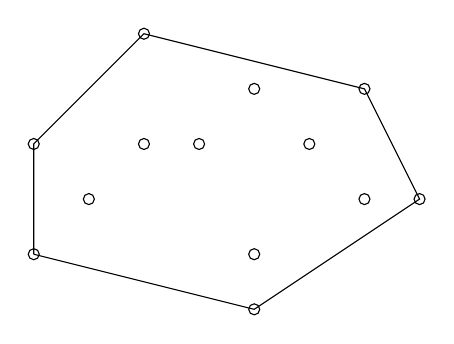
\begin{tikzpicture}[scale=0.7]
        \draw (0,0)--(4,-1)--(7,1)--(6,3)--(2,4)--(0,2)--(0,0);

        \draw (0,0) circle [radius=0.1];
        \draw (4,-1) circle [radius=0.1];
        \draw (7,1) circle [radius=0.1];
        \draw (6,3) circle [radius=0.1];
        \draw (2,4) circle [radius=0.1];
        \draw (0,2) circle [radius=0.1];

        \draw (1,1) circle [radius=0.1];
        \draw (2,2) circle [radius=0.1];
        \draw (3,2) circle [radius=0.1];
        \draw (4,0) circle [radius=0.1];
        \draw (4,3) circle [radius=0.1];
        \draw (5,2) circle [radius=0.1];
        \draw (6,1) circle [radius=0.1];
    \end{tikzpicture}
\end{center}

\index{algoritmo de!Andrew}

El \key{algoritmo de Andrew} \cite{and79} nos da una manera fácil de construir
la envolvente convexa de un conjunto de puntos en $O(n \log n)$. Primero, el
algoritmo ubica los puntos más a la izquierda y a la derecha, y luego
construye la envolvente en dos partes: primero la envolvente superior y luego
la envolvente inferior. Ambas partes son similares, por lo que nos podemos
concentrar en la superior.

Primero, ordenamos los puntos principalmente por sus coordenadas $x$ y
secundariamente por sus coordenadas $y$. Luego de esto, recorremos los
puntos y añadimos cada punto a la envolvente. Siempre, luego de añadir
un punto a la envolvente, nos aseguramos de que el último segmento no
gire a la izquierda. Mientras gire a la izquierda, removemos el
anteúltimo punto de la envolvente repetidamente.

La siguiente imagen muestra el funcionamiento del algoritmo de Andrew:
\\
\begin{tabular}{ccccccc}
    \\
    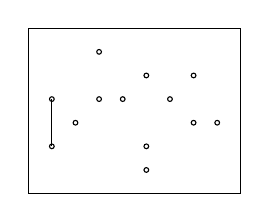
\begin{tikzpicture}[scale=0.3]
        \draw (-1,-2)--(8,-2)--(8,5)--(-1,5)--(-1,-2);
        \draw (0,0) circle [radius=0.1];
        \draw (4,-1) circle [radius=0.1];
        \draw (7,1) circle [radius=0.1];
        \draw (6,3) circle [radius=0.1];
        \draw (2,4) circle [radius=0.1];
        \draw (0,2) circle [radius=0.1];

        \draw (1,1) circle [radius=0.1];
        \draw (2,2) circle [radius=0.1];
        \draw (3,2) circle [radius=0.1];
        \draw (4,0) circle [radius=0.1];
        \draw (4,3) circle [radius=0.1];
        \draw (5,2) circle [radius=0.1];
        \draw (6,1) circle [radius=0.1];

        \draw (0,0)--(0,2);
    \end{tikzpicture}
      & \hspace{0.1cm} &
    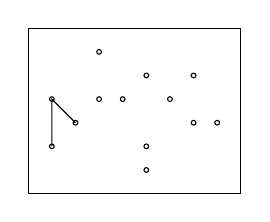
\begin{tikzpicture}[scale=0.3]
        \draw (-1,-2)--(8,-2)--(8,5)--(-1,5)--(-1,-2);
        \draw (0,0) circle [radius=0.1];
        \draw (4,-1) circle [radius=0.1];
        \draw (7,1) circle [radius=0.1];
        \draw (6,3) circle [radius=0.1];
        \draw (2,4) circle [radius=0.1];
        \draw (0,2) circle [radius=0.1];

        \draw (1,1) circle [radius=0.1];
        \draw (2,2) circle [radius=0.1];
        \draw (3,2) circle [radius=0.1];
        \draw (4,0) circle [radius=0.1];
        \draw (4,3) circle [radius=0.1];
        \draw (5,2) circle [radius=0.1];
        \draw (6,1) circle [radius=0.1];

        \draw (0,0)--(0,2)--(1,1);
    \end{tikzpicture}
      & \hspace{0.1cm} &
    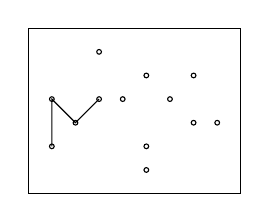
\begin{tikzpicture}[scale=0.3]
        \draw (-1,-2)--(8,-2)--(8,5)--(-1,5)--(-1,-2);
        \draw (0,0) circle [radius=0.1];
        \draw (4,-1) circle [radius=0.1];
        \draw (7,1) circle [radius=0.1];
        \draw (6,3) circle [radius=0.1];
        \draw (2,4) circle [radius=0.1];
        \draw (0,2) circle [radius=0.1];

        \draw (1,1) circle [radius=0.1];
        \draw (2,2) circle [radius=0.1];
        \draw (3,2) circle [radius=0.1];
        \draw (4,0) circle [radius=0.1];
        \draw (4,3) circle [radius=0.1];
        \draw (5,2) circle [radius=0.1];
        \draw (6,1) circle [radius=0.1];

        \draw (0,0)--(0,2)--(1,1)--(2,2);
    \end{tikzpicture}
      & \hspace{0.1cm} &
    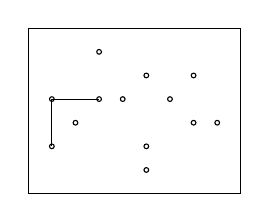
\begin{tikzpicture}[scale=0.3]
        \draw (-1,-2)--(8,-2)--(8,5)--(-1,5)--(-1,-2);
        \draw (0,0) circle [radius=0.1];
        \draw (4,-1) circle [radius=0.1];
        \draw (7,1) circle [radius=0.1];
        \draw (6,3) circle [radius=0.1];
        \draw (2,4) circle [radius=0.1];
        \draw (0,2) circle [radius=0.1];

        \draw (1,1) circle [radius=0.1];
        \draw (2,2) circle [radius=0.1];
        \draw (3,2) circle [radius=0.1];
        \draw (4,0) circle [radius=0.1];
        \draw (4,3) circle [radius=0.1];
        \draw (5,2) circle [radius=0.1];
        \draw (6,1) circle [radius=0.1];

        \draw (0,0)--(0,2)--(2,2);
    \end{tikzpicture}
    \\
    1 &                & 2 &  & 3 &  & 4 \\
\end{tabular}
\\
\begin{tabular}{ccccccc}
    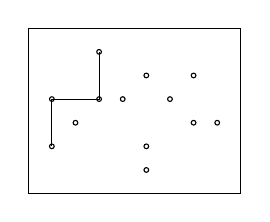
\begin{tikzpicture}[scale=0.3]
        \draw (-1,-2)--(8,-2)--(8,5)--(-1,5)--(-1,-2);
        \draw (0,0) circle [radius=0.1];
        \draw (4,-1) circle [radius=0.1];
        \draw (7,1) circle [radius=0.1];
        \draw (6,3) circle [radius=0.1];
        \draw (2,4) circle [radius=0.1];
        \draw (0,2) circle [radius=0.1];

        \draw (1,1) circle [radius=0.1];
        \draw (2,2) circle [radius=0.1];
        \draw (3,2) circle [radius=0.1];
        \draw (4,0) circle [radius=0.1];
        \draw (4,3) circle [radius=0.1];
        \draw (5,2) circle [radius=0.1];
        \draw (6,1) circle [radius=0.1];

        \draw (0,0)--(0,2)--(2,2)--(2,4);
    \end{tikzpicture}
      & \hspace{0.1cm} &
    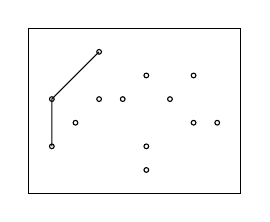
\begin{tikzpicture}[scale=0.3]
        \draw (-1,-2)--(8,-2)--(8,5)--(-1,5)--(-1,-2);
        \draw (0,0) circle [radius=0.1];
        \draw (4,-1) circle [radius=0.1];
        \draw (7,1) circle [radius=0.1];
        \draw (6,3) circle [radius=0.1];
        \draw (2,4) circle [radius=0.1];
        \draw (0,2) circle [radius=0.1];

        \draw (1,1) circle [radius=0.1];
        \draw (2,2) circle [radius=0.1];
        \draw (3,2) circle [radius=0.1];
        \draw (4,0) circle [radius=0.1];
        \draw (4,3) circle [radius=0.1];
        \draw (5,2) circle [radius=0.1];
        \draw (6,1) circle [radius=0.1];

        \draw (0,0)--(0,2)--(2,4);
    \end{tikzpicture}
      & \hspace{0.1cm} &
    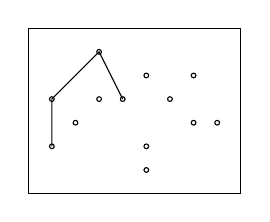
\begin{tikzpicture}[scale=0.3]
        \draw (-1,-2)--(8,-2)--(8,5)--(-1,5)--(-1,-2);
        \draw (0,0) circle [radius=0.1];
        \draw (4,-1) circle [radius=0.1];
        \draw (7,1) circle [radius=0.1];
        \draw (6,3) circle [radius=0.1];
        \draw (2,4) circle [radius=0.1];
        \draw (0,2) circle [radius=0.1];

        \draw (1,1) circle [radius=0.1];
        \draw (2,2) circle [radius=0.1];
        \draw (3,2) circle [radius=0.1];
        \draw (4,0) circle [radius=0.1];
        \draw (4,3) circle [radius=0.1];
        \draw (5,2) circle [radius=0.1];
        \draw (6,1) circle [radius=0.1];

        \draw (0,0)--(0,2)--(2,4)--(3,2);
    \end{tikzpicture}
      & \hspace{0.1cm} &
    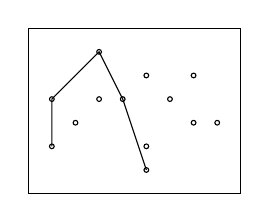
\begin{tikzpicture}[scale=0.3]
        \draw (-1,-2)--(8,-2)--(8,5)--(-1,5)--(-1,-2);
        \draw (0,0) circle [radius=0.1];
        \draw (4,-1) circle [radius=0.1];
        \draw (7,1) circle [radius=0.1];
        \draw (6,3) circle [radius=0.1];
        \draw (2,4) circle [radius=0.1];
        \draw (0,2) circle [radius=0.1];

        \draw (1,1) circle [radius=0.1];
        \draw (2,2) circle [radius=0.1];
        \draw (3,2) circle [radius=0.1];
        \draw (4,0) circle [radius=0.1];
        \draw (4,3) circle [radius=0.1];
        \draw (5,2) circle [radius=0.1];
        \draw (6,1) circle [radius=0.1];

        \draw (0,0)--(0,2)--(2,4)--(3,2)--(4,-1);
    \end{tikzpicture}
    \\
    5 &                & 6 &  & 7 &  & 8 \\
\end{tabular}
\\
\begin{tabular}{ccccccc}
    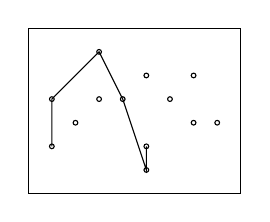
\begin{tikzpicture}[scale=0.3]
        \draw (-1,-2)--(8,-2)--(8,5)--(-1,5)--(-1,-2);
        \draw (0,0) circle [radius=0.1];
        \draw (4,-1) circle [radius=0.1];
        \draw (7,1) circle [radius=0.1];
        \draw (6,3) circle [radius=0.1];
        \draw (2,4) circle [radius=0.1];
        \draw (0,2) circle [radius=0.1];

        \draw (1,1) circle [radius=0.1];
        \draw (2,2) circle [radius=0.1];
        \draw (3,2) circle [radius=0.1];
        \draw (4,0) circle [radius=0.1];
        \draw (4,3) circle [radius=0.1];
        \draw (5,2) circle [radius=0.1];
        \draw (6,1) circle [radius=0.1];

        \draw (0,0)--(0,2)--(2,4)--(3,2)--(4,-1)--(4,0);
    \end{tikzpicture}
      & \hspace{0.1cm} &
    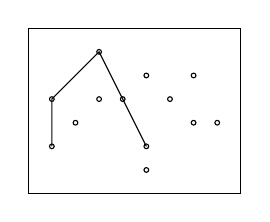
\begin{tikzpicture}[scale=0.3]
        \draw (-1,-2)--(8,-2)--(8,5)--(-1,5)--(-1,-2);
        \draw (0,0) circle [radius=0.1];
        \draw (4,-1) circle [radius=0.1];
        \draw (7,1) circle [radius=0.1];
        \draw (6,3) circle [radius=0.1];
        \draw (2,4) circle [radius=0.1];
        \draw (0,2) circle [radius=0.1];

        \draw (1,1) circle [radius=0.1];
        \draw (2,2) circle [radius=0.1];
        \draw (3,2) circle [radius=0.1];
        \draw (4,0) circle [radius=0.1];
        \draw (4,3) circle [radius=0.1];
        \draw (5,2) circle [radius=0.1];
        \draw (6,1) circle [radius=0.1];

        \draw (0,0)--(0,2)--(2,4)--(3,2)--(4,0);
    \end{tikzpicture}
      & \hspace{0.1cm} &
    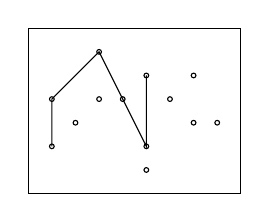
\begin{tikzpicture}[scale=0.3]
        \draw (-1,-2)--(8,-2)--(8,5)--(-1,5)--(-1,-2);
        \draw (0,0) circle [radius=0.1];
        \draw (4,-1) circle [radius=0.1];
        \draw (7,1) circle [radius=0.1];
        \draw (6,3) circle [radius=0.1];
        \draw (2,4) circle [radius=0.1];
        \draw (0,2) circle [radius=0.1];

        \draw (1,1) circle [radius=0.1];
        \draw (2,2) circle [radius=0.1];
        \draw (3,2) circle [radius=0.1];
        \draw (4,0) circle [radius=0.1];
        \draw (4,3) circle [radius=0.1];
        \draw (5,2) circle [radius=0.1];
        \draw (6,1) circle [radius=0.1];

        \draw (0,0)--(0,2)--(2,4)--(3,2)--(4,0)--(4,3);
    \end{tikzpicture}
      & \hspace{0.1cm} &
    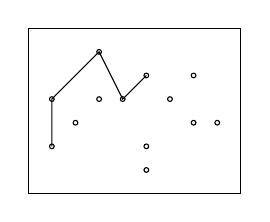
\begin{tikzpicture}[scale=0.3]
        \draw (-1,-2)--(8,-2)--(8,5)--(-1,5)--(-1,-2);
        \draw (0,0) circle [radius=0.1];
        \draw (4,-1) circle [radius=0.1];
        \draw (7,1) circle [radius=0.1];
        \draw (6,3) circle [radius=0.1];
        \draw (2,4) circle [radius=0.1];
        \draw (0,2) circle [radius=0.1];

        \draw (1,1) circle [radius=0.1];
        \draw (2,2) circle [radius=0.1];
        \draw (3,2) circle [radius=0.1];
        \draw (4,0) circle [radius=0.1];
        \draw (4,3) circle [radius=0.1];
        \draw (5,2) circle [radius=0.1];
        \draw (6,1) circle [radius=0.1];

        \draw (0,0)--(0,2)--(2,4)--(3,2)--(4,3);
    \end{tikzpicture}
    \\
    9 &                & 10 &  & 11 &  & 12 \\
\end{tabular}
\\
\begin{tabular}{ccccccc}
    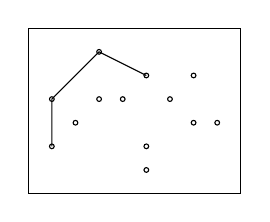
\begin{tikzpicture}[scale=0.3]
        \draw (-1,-2)--(8,-2)--(8,5)--(-1,5)--(-1,-2);
        \draw (0,0) circle [radius=0.1];
        \draw (4,-1) circle [radius=0.1];
        \draw (7,1) circle [radius=0.1];
        \draw (6,3) circle [radius=0.1];
        \draw (2,4) circle [radius=0.1];
        \draw (0,2) circle [radius=0.1];

        \draw (1,1) circle [radius=0.1];
        \draw (2,2) circle [radius=0.1];
        \draw (3,2) circle [radius=0.1];
        \draw (4,0) circle [radius=0.1];
        \draw (4,3) circle [radius=0.1];
        \draw (5,2) circle [radius=0.1];
        \draw (6,1) circle [radius=0.1];

        \draw (0,0)--(0,2)--(2,4)--(4,3);
    \end{tikzpicture}
       & \hspace{0.1cm} &
    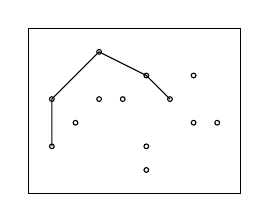
\begin{tikzpicture}[scale=0.3]
        \draw (-1,-2)--(8,-2)--(8,5)--(-1,5)--(-1,-2);
        \draw (0,0) circle [radius=0.1];
        \draw (4,-1) circle [radius=0.1];
        \draw (7,1) circle [radius=0.1];
        \draw (6,3) circle [radius=0.1];
        \draw (2,4) circle [radius=0.1];
        \draw (0,2) circle [radius=0.1];

        \draw (1,1) circle [radius=0.1];
        \draw (2,2) circle [radius=0.1];
        \draw (3,2) circle [radius=0.1];
        \draw (4,0) circle [radius=0.1];
        \draw (4,3) circle [radius=0.1];
        \draw (5,2) circle [radius=0.1];
        \draw (6,1) circle [radius=0.1];

        \draw (0,0)--(0,2)--(2,4)--(4,3)--(5,2);
    \end{tikzpicture}
       & \hspace{0.1cm} &
    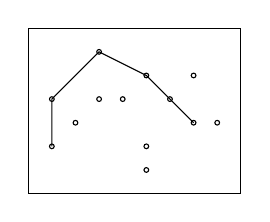
\begin{tikzpicture}[scale=0.3]
        \draw (-1,-2)--(8,-2)--(8,5)--(-1,5)--(-1,-2);
        \draw (0,0) circle [radius=0.1];
        \draw (4,-1) circle [radius=0.1];
        \draw (7,1) circle [radius=0.1];
        \draw (6,3) circle [radius=0.1];
        \draw (2,4) circle [radius=0.1];
        \draw (0,2) circle [radius=0.1];

        \draw (1,1) circle [radius=0.1];
        \draw (2,2) circle [radius=0.1];
        \draw (3,2) circle [radius=0.1];
        \draw (4,0) circle [radius=0.1];
        \draw (4,3) circle [radius=0.1];
        \draw (5,2) circle [radius=0.1];
        \draw (6,1) circle [radius=0.1];

        \draw (0,0)--(0,2)--(2,4)--(4,3)--(5,2)--(6,1);
    \end{tikzpicture}
       & \hspace{0.1cm} &
    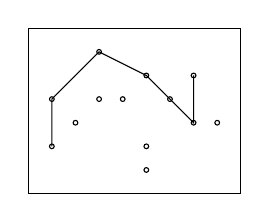
\begin{tikzpicture}[scale=0.3]
        \draw (-1,-2)--(8,-2)--(8,5)--(-1,5)--(-1,-2);
        \draw (0,0) circle [radius=0.1];
        \draw (4,-1) circle [radius=0.1];
        \draw (7,1) circle [radius=0.1];
        \draw (6,3) circle [radius=0.1];
        \draw (2,4) circle [radius=0.1];
        \draw (0,2) circle [radius=0.1];

        \draw (1,1) circle [radius=0.1];
        \draw (2,2) circle [radius=0.1];
        \draw (3,2) circle [radius=0.1];
        \draw (4,0) circle [radius=0.1];
        \draw (4,3) circle [radius=0.1];
        \draw (5,2) circle [radius=0.1];
        \draw (6,1) circle [radius=0.1];

        \draw (0,0)--(0,2)--(2,4)--(4,3)--(5,2)--(6,1)--(6,3);
    \end{tikzpicture}
    \\
    13 &                & 14 &  & 15 &  & 16 \\
\end{tabular}
\\
\begin{tabular}{ccccccc}
    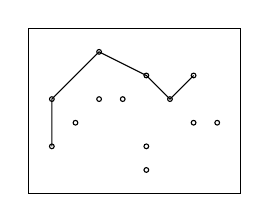
\begin{tikzpicture}[scale=0.3]
        \draw (-1,-2)--(8,-2)--(8,5)--(-1,5)--(-1,-2);
        \draw (0,0) circle [radius=0.1];
        \draw (4,-1) circle [radius=0.1];
        \draw (7,1) circle [radius=0.1];
        \draw (6,3) circle [radius=0.1];
        \draw (2,4) circle [radius=0.1];
        \draw (0,2) circle [radius=0.1];

        \draw (1,1) circle [radius=0.1];
        \draw (2,2) circle [radius=0.1];
        \draw (3,2) circle [radius=0.1];
        \draw (4,0) circle [radius=0.1];
        \draw (4,3) circle [radius=0.1];
        \draw (5,2) circle [radius=0.1];
        \draw (6,1) circle [radius=0.1];

        \draw (0,0)--(0,2)--(2,4)--(4,3)--(5,2)--(6,3);
    \end{tikzpicture}
       & \hspace{0.1cm} &
    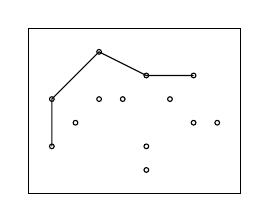
\begin{tikzpicture}[scale=0.3]
        \draw (-1,-2)--(8,-2)--(8,5)--(-1,5)--(-1,-2);
        \draw (0,0) circle [radius=0.1];
        \draw (4,-1) circle [radius=0.1];
        \draw (7,1) circle [radius=0.1];
        \draw (6,3) circle [radius=0.1];
        \draw (2,4) circle [radius=0.1];
        \draw (0,2) circle [radius=0.1];

        \draw (1,1) circle [radius=0.1];
        \draw (2,2) circle [radius=0.1];
        \draw (3,2) circle [radius=0.1];
        \draw (4,0) circle [radius=0.1];
        \draw (4,3) circle [radius=0.1];
        \draw (5,2) circle [radius=0.1];
        \draw (6,1) circle [radius=0.1];

        \draw (0,0)--(0,2)--(2,4)--(4,3)--(6,3);
    \end{tikzpicture}
       & \hspace{0.1cm} &
    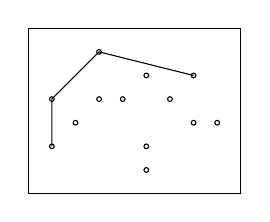
\begin{tikzpicture}[scale=0.3]
        \draw (-1,-2)--(8,-2)--(8,5)--(-1,5)--(-1,-2);
        \draw (0,0) circle [radius=0.1];
        \draw (4,-1) circle [radius=0.1];
        \draw (7,1) circle [radius=0.1];
        \draw (6,3) circle [radius=0.1];
        \draw (2,4) circle [radius=0.1];
        \draw (0,2) circle [radius=0.1];

        \draw (1,1) circle [radius=0.1];
        \draw (2,2) circle [radius=0.1];
        \draw (3,2) circle [radius=0.1];
        \draw (4,0) circle [radius=0.1];
        \draw (4,3) circle [radius=0.1];
        \draw (5,2) circle [radius=0.1];
        \draw (6,1) circle [radius=0.1];

        \draw (0,0)--(0,2)--(2,4)--(6,3);
    \end{tikzpicture}
       & \hspace{0.1cm} &
    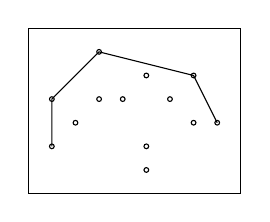
\begin{tikzpicture}[scale=0.3]
        \draw (-1,-2)--(8,-2)--(8,5)--(-1,5)--(-1,-2);
        \draw (0,0) circle [radius=0.1];
        \draw (4,-1) circle [radius=0.1];
        \draw (7,1) circle [radius=0.1];
        \draw (6,3) circle [radius=0.1];
        \draw (2,4) circle [radius=0.1];
        \draw (0,2) circle [radius=0.1];

        \draw (1,1) circle [radius=0.1];
        \draw (2,2) circle [radius=0.1];
        \draw (3,2) circle [radius=0.1];
        \draw (4,0) circle [radius=0.1];
        \draw (4,3) circle [radius=0.1];
        \draw (5,2) circle [radius=0.1];
        \draw (6,1) circle [radius=0.1];

        \draw (0,0)--(0,2)--(2,4)--(6,3)--(7,1);
    \end{tikzpicture}
    \\
    17 &                & 18 &  & 19 &  & 20
\end{tabular}




